\documentclass[11pt, letterpaper]{article}
\usepackage{common, comment}
\usepackage{amsmath}
\usepackage{setspace}
\usepackage{graphicx}
\usepackage{tikz}
\tikzset{> = latex, every picture/.style={line width=0.7pt}}

% \pdfpagewidth 8.5in
% \pdfpageheight 11in 

% \setlength\topmargin{0in}
% \setlength\headheight{0in}
% \setlength\headsep{0in}
% \setlength\textheight{9in}
% \setlength\textwidth{5.5in}
% \setlength\oddsidemargin{.5in}
% \setlength\evensidemargin{.5in}
% \setlength\parindent{0.25in}
% \setlength\parskip{0in}
\usepackage[margin=1in]{geometry}

% Solution environment
\newenvironment{solution}
  {\color{blue}\section*{Solution}}
{}

\excludecomment{solution} % UNCOMMENT TO HIDE SOLUTIONS


\begin{document}
\begin{center}
    {\LARGE CS 181 Spring 2024 Section 10:\\
        {\Large Reinforcement Learning }}
\end{center}

\section{Introduction}

In the reinforcement learning setting, unlike MDPs, we don't have direct access to the transition distribution $p(s'|s,a)$ or the reward function $r(s,a)$ --- information about these only come to us through the outcome of the environment. 
This problem is hard because some states can lead to high rewards, but we don't know which ones; even if we did, we don't know how to get there!

To deal with this, in lecture, we discussed \textit{model-based} and \textit{model-free} reinforcement learning. 


\section{From Planning to Reinforcement Learning}

Recall that MDPs are defined by a set of states, actions, rewards, and
transition probabilities $\{S, A, r, p\}$, and our goal is to find the
policy $\pi^\ast$ that maximizes the expected sum of discounted rewards.

In planning, we are explicitly provided with  the model of the environment, whereas in reinforcement learning, an agent does not have a model of the environment to begin with. Instead, it must interact with the environment to learn what its policy should be. 

\subsection{Concept Question}

Would the following be problems more likely to be solved with MDP planning
and which through  reinforcement learning?
%
\begin{enumerate}
    \item Finding the best route to take through a treacherous forest using a map. 
    
    \item Bringing the new Boston Dynamics robot into a new obstacle course it has never seen before. 
\end{enumerate}

\begin{solution}
\begin{enumerate}
    \item \boxed{\text{MDP Planning}}, as we are given the $\{S, A, r, p\}$ formulations through the map.
    \item \boxed{\text{Reinforcement Learning}}, since we initialize start off with little to no knowledge about the environment, and therefore cannot solve some pre-defined MDP.
\end{enumerate}
\end{solution}

\section{Model-based Learning}

For model-based learning, we estimate the missing world models: $r(s, a)$ and $p(s'|s, a)$, and then use planning (value or policy iteration) to develop a policy $\pi$. 

\subsection{Concept Question}

Can you think of a way to do this in practice? What are some
downsides?

\begin{solution}
\begin{itemize}
    \item  One way to do this is to perform a number of random walks (at
  each state, we take a random action, and we track the rewards we get
  and the states we transition to). 
  
  For the transition model, we maintain counts on different next states
  given $(s,a)$ pairs, and we use this to update a Dirichlet model for
  the distribution on $p(\cdot|s,a)$ for each $s,a$). For the reward model,
  one simple approach would be to track the average reward achieved
  for each state-action pair.

  We can then use the transition and reward models for planning. We would act according to the obtained plan, perhaps adding some $\epsilon$-greedy exploration. This will give us more environmental interaction data, and we can use it to update our reward and transition models.
  %
\item A downside to model-based RL can be that
  it's unnecessarily complex--- suppose there are many states, in
  which case the transition model $p(s'|s,a)$ becomes huge, and it may
  be hard to get a good estimate of the true model.
This can make model-based learning inefficient and 
difficult to generalize.

Also, recall that  the goal is not to learn the
  transition model. Rather,  it is to learn an optimal policy, and so we may be
  doing unnecessary work.
\end{itemize} 
\end{solution}

\vspace{.5pc}

\section{Model-Free Learning}

In model-free learning, we are no longer interested in learning the
transition function and reward function. Instead, we are looking to
directly infer the optimal policy from samples of the world --- that
is, given that we are in state $s$, we want to know the best action
$a = \pi^*(s)$ to take. This makes model-free learning cheaper and
simpler.

To do this, we look to learn the optimal Q-values, defined as
%
\begin{align}
  Q^*(s,a)=r(s,a)+\gamma\sum_{s' \in S}p(s' | s, a) V^*(s'), \text{
  } \forall s,a
\end{align}
where $V^*(s)$ is the optimal value function.  The value $Q^*(s,a)$ is
the value from taking action $a$ in state $s$ and then following the
optimal continuation from the next state.

By learning this Q-value function, $Q^*$, we also have the optimal
policy, with
%
\begin{align}
    \pi^*(s) = \argmax_aQ^*(s, a)
\end{align}

To learn $Q^*$ we can perform a one-step decomposition, and we get an
alternate form of the Bellman equations which states that for an
optimal policy $\pi^*$,
%
\begin{align}
    Q^*(s,a) = r(s,a) + \gamma\sum_{s' \in S}p(s' | s, a)\max_{a' \in A}[Q^*(s', a')], \text{  } \forall s,a \label{eq:q_bellman}
\end{align}


Intuitively, for an optimal policy, the Q value at the current state and action should be equivalent to the current reward plus the \emph{maximum} possible expected future value from the next state. 


The question then becomes how we can find the Q values that satisfy the Bellman equations as written in Equation~\ref{eq:q_bellman}. There are two ways that we do this. One is ``on-policy'' (SARSA) and one is ``off-policy'' (Q-learning).

% This is where the optional material used to be, but moved to the back for the sake of time

\subsection{Q Values Example}
\begin{figure}[!h]
  \centering
  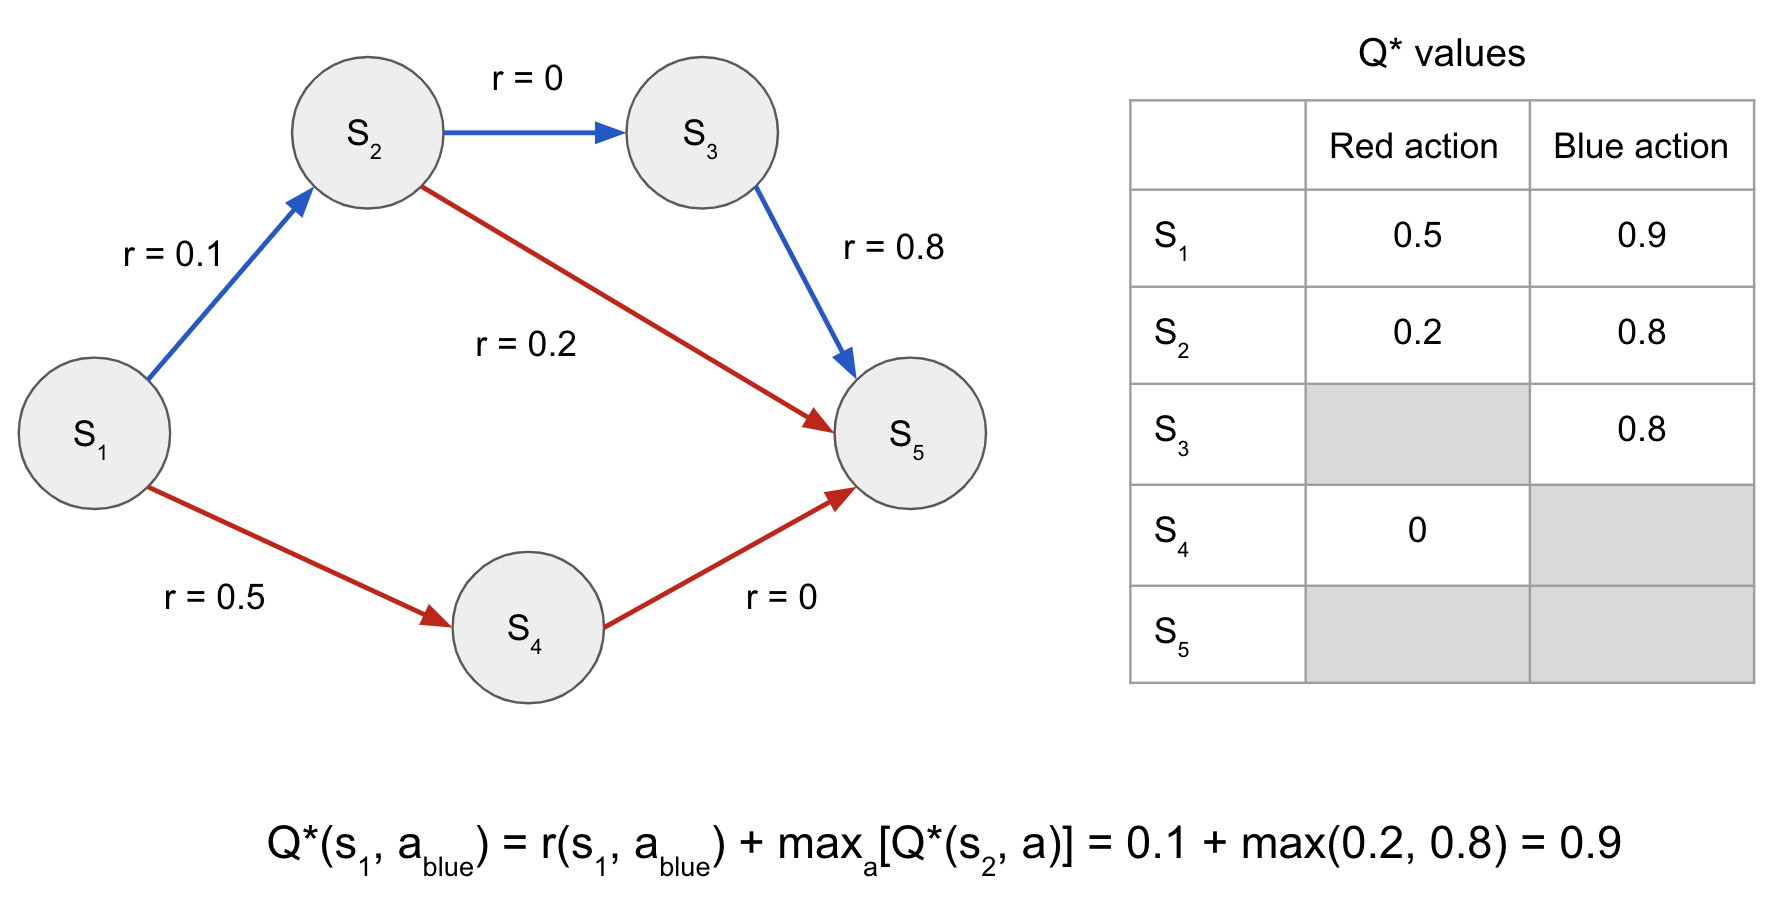
\includegraphics[width=1.0\linewidth]{optimal_qs_example.png}
\end{figure}

In the above figure, suppose that the discount factor is 1.0 and the actions are deterministic. The agent starts from state $s_1$ and will finish in the state $s_5$, from which no more actions are taken. We can represent Q values as a table of states and actions, as shown to the right. For these converged Q values (corresponding to an optimal policy), we can quickly verify that the Q value of a given state and action is the sum of the current reward and the maximum of the Q value from the next state. We can read the optimal policy off the table by selecting the action that maximizes the value of a given state. For example, in state 1, we should take the blue action.  

\subsection{Exploration vs. Exploitation}

An RL agent also needs to decide how to act in the environment while
collecting observations. This gets to the
key issue of \emph{exploration vs. exploitation}.

In an exploitative approach, when we are in state $s$, we can simply
take action $a = \argmax_{a \in A} Q(s,a)$ based on our current
estimate of the Q-function.

In an explorative approach, we want to ensure that we have visited
enough states and taken enough actions from those states to get good
Q-function estimates, and this can lead us to prefer to add some
randomization to the behavior of the agent.

\subsubsection{Concept Question}

What would be a problem if our approach was only exploitative? In
practice, how might we balance exploitation vs exploration?
%
\begin{solution}
\begin{itemize}
\item If we focus on exploitation and do not explore enough,
    we might end up with a bad estimate of the Q-function and never
    find the true best action. We want to balance these two---
    exploitation  is a policy that is following the advice of the
    Q-value estimates and useful when this knowledge is good,
    while exploration is necessary to properly understand the MDP. Referring back to example 4.1, we see that if we had not sufficiently explored from state 1, then the red action seems to be better to take than the blue action, which actually results in the higher overall value.
%
\item In practice, $\epsilon$-greedy is a sensible approach
    for allowing an RL agent to explore and exploit while learning in an
    unknown environment.
    %
    In the $\epsilon$-greedy method, we take $\argmax_{a \in A} Q(s,a)$ with probability $1-\epsilon$, and pick $a \in A$ uniformly at random with probability $\epsilon$ (for some $\epsilon>0$).
%
\end{itemize}
\end{solution}

\section{On-Policy RL: SARSA}

Whatever the behavior of the RL agent, a first way to update the 
Q-values is
an \emph{on-policy} method.

Given current state $s$, current
action $a$, reward $r$, next state $s'$, next action $a'$
($s,a,r,s',a$, hence the name SARSA), the update is
%
%
\begin{align}
    Q(s,a) \leftarrow Q(s,a) + \alpha_t\left[ r + \gamma Q(s', a') - Q(s,a)\right]
\end{align}

This is known as the SARSA update (State-Action-Reward-State-Action),
since we look ahead to get the action $\pi(s')$.  Here, $\alpha_t$,
with $0\leq \alpha_t<1$ is the learning rate at update $t$.
$\gamma$ is the discount factor. $a'$ is chosen thorugh the $\epsilon$-greedy method.

Here, we are taking the difference between our current $Q$-value at a
state-action and the one that we predict using the current reward and the
discounted Q-value following the policy. We update the $Q(s,a)$ value
in the direction of this difference, which is known as the ``temporal
difference error.''

Since we follow $\pi$ in choosing action $a'$, this gradient method is
on-policy. In particular, it learns Q-values that correspond to the
behavior of the agent. The SARSA update rule is like we're doing a
stochastic gradient descent for one observation, looking to improve
our estimate of $Q(s,a)$.

Because SARSA is on-policy, it is not guranteed to converge to the
optimal Q-values. In order to converge to the optimal Q-values, SARSA
needs to (stated informally):
%
\begin{itemize}
\item Visit every action in every state infinitely often,
\item Decay the learning rate over time, but not too
             quickly,\footnote{For each $(s,a)$ pair, we need
             $\sum_t \alpha_t=\infty$ for the periods $t$ in which we
             update $Q(s,a)$ (don't reduce learning rate too quickly),
             and $\sum_t\alpha_t^2<\infty$ (eventually learning rate
             becomes small). A typical choice is to set the  learning rate
    $\alpha_t$ for an update on $(s,a)$  to $1/N(s,a)$ where
    $N(s,a)$ is the number of times action $a$ is taken in state $s$.}
  %
    \item Move from $\epsilon$-greedy to greedy over time, so that in
      the limit the policy is greedy; e.g., it can be useful to set
      $\epsilon$ for a state $s$ to $c/N(s)$ where $N(s)$ is the
      number of times the state has been visited.
      \end{itemize}


      \subsection{Concept Question}

      What would SARSA learn when following a fixed policy $\pi$? What
      is the tension in reducing exploration $\epsilon$ in
      $\epsilon$-greedy when using SARSA to learn the optimal $Q^*$ values?
      %

\begin{solution}
      \begin{itemize}
      \item  The Q-values corresponding to policy $\pi$, i.e.
          \begin{align}
           Q^\pi(s,a)&=r(s,a)+\gamma\sum_{s'}p(s'|s,a)Q^\pi(s',\pi(s'))
        \end{align}
      \item The tension with SARSA  is that we need to both visit every
          action in every state infinitely often (explore) but also
          eventually stop adding random exploration (exploit). This is
        often called GLIE ``greedy in the limit of infinite exploration.''
      \end{itemize}
\end{solution}

\section{Off-Policy RL: Q-Learning}

Whatever the behavior of the RL agent, a second way to update the
Q-values is an \emph{off-policy} method. 


Given current state $s$, current action $a$, reward $r$, next state
$s'$, the update in Q-learning is:
%
%
\begin{align}
  Q(s,a) & \leftarrow  Q(s,a)+\alpha_t[r +\gamma
           \max_{a'}Q(s',a')-Q(s,a)]
           \end{align}

           Q-learning uses State-Action-Reward-State from the
           environment.  It is the max over actions $a'$ that makes
          this an `off-policy' method.
          Here, we are taking the difference between our current $Q$-value
          for a state-action and the one that we predict using the
          current reward and the discounted $Q$-value when following
          the best action from the next state. 
          We update the $Q(s,a)$ value to reduce this difference,
          which is known as the ``temporal difference error.''

          We can see that the Q-learning update can be viewed as a
          stochastic gradient descent for one observation, looking to
          find estimates of $Q$-values that better approximate the
          Bellman equations.

           Because Q-learning is off policy, it is guaranteed to
           converge to the optimal $Q$-values as long as the following
           is true (stated informally):
           %
           \begin{itemize}
           \item Visit every action in every state infinitely often
           \item Decay the learning rate over time, but not too
             quickly.\footnote{For each $(s,a)$ pair, we need
             $\sum_t \alpha_t=\infty$ for the periods $t$ in which we
             update $Q(s,a)$ (don't reduce learning rate too quickly),
             and $\sum_t\alpha_t^2<\infty$ (eventually learning rate
             becomes small). A typical choice is to set the  learning rate
    $\alpha_t$ for an update on $(s,a)$  to $1/N(s,a)$ where
    $N(s,a)$ is the number of times action $a$ is taken in state $s$.}
  \end{itemize}


  \subsection{Concept Question}

  Is the Q-learning update equal to the SARSA learning update in the
  case that the behavior in SARSA is greedy and not $\epsilon$-greedy?
%
\begin{solution}
      \begin{itemize}
  \item Yes! In this case, we can easily check that the two
      update equations are equivalent because the next state action
      used  in the  SARSA update is $\max_{a'}Q(s',a')$, which is the same
      as in the Q-learning update.
  \end{itemize}
\end{solution}

\section{Exercise: Model-free RL}

\noindent \fbox{\parbox{\linewidth}{%
    Consider the same MDP below on the following grid. 
    
    \begin{center}
    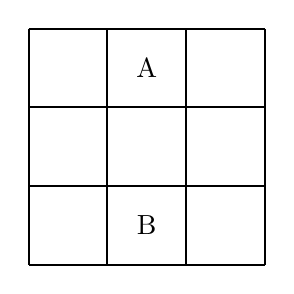
\begin{tikzpicture}
    \draw[step=1cm] (-2,-2) grid (1,1);
    \node at (-0.5,+0.5) {A};
    \node at (-0.5,-1.5) {B};
    \end{tikzpicture}
    \end{center}
    
    At each square, we can go left, right, up, or down. Normally we get a reward of 0 from moving, but if we attempt to move off the grid, we get a reward of $-1$ and stay where we are. Also, if we move onto square A, we get a reward of 10 and are teleported to square B. The discount factor is $\gamma=0.9$. \\
    
   % However, suppose now we are in the reinforcement learning setting,
   % where we don't know the transition probabilities $p(s'|s,a)$ or
    %the reward function $r(s,a)$.

Suppose an RL agent starts at the top left square, $(0,0)$, and follow an
$\epsilon$-greedy policy. At the beginning, suppose $Q(s,a) = 0$ for all $s,a$, except we know that we shouldn't go off the grid, so that the values of $Q$ for the corresponding $s,a$ pairs are $-1$ (ie. moving off the grid from position $(0,0)$ to $(-1,0)$ is disallowed and corresponds with an initialization of $Q(s,a)=-1$). \\

The learning rate $\alpha = 0.1$.  With RL, the realized reward for an action will depend on the state, the action, and whether or not the action succeeds.

%
\begin{enumerate}
\item For the first step, suppose $\epsilon$-greedy tells
  the agent to explore, and the agent selects right as its action (and
  this action succeeds).  Write the Q-learning update in step one.
      %
\item Now write the SARSA update for step one, assuming that in
  addition to right in step one, $\epsilon$-greedy tells
  the agent to explore and go down in the second step (and this action
  succeeds).
  %

  \item Are the updates the same? If not, why not?
\end{enumerate}

}}

\vspace{0.5pc}

\begin{solution}
 
\begin{enumerate}
\item Our environment gives us $r = 10$ for succeeding with the right
  action, and $s' = (2,1)$ for the next state.
%
  For Q-learning, we can use this first step
  and next state to update the value of $Q(s,a)$ for $s=(0,0)$,
action   $a=\text{R}$, and next state $s'=(2,1)$  as follows
%
\begin{align}
  Q(s,a)&\leftarrow Q(s,a)+\alpha(r+\gamma\max_{a'}Q(s',a')-Q(s,a))
  \\
        &=0 + (0.1)(10+0.9\max\{0,-1,0,0\}-0) = 1
\end{align}

\item With knowledge that in next 
  state $s'=(2,1)$ the action $a'$ is down, the SARSA method will
  update the $Q$-value for state $s=(0,0)$ and action $a=$ right as follows
  %
  \begin{align}
    Q(s,a)&\leftarrow Q(s,a)+\alpha(r+Q(s',a')-Q(s,a))\\
    &=0+(0.1)(10+(0.9)(-1)-0)=0.1(10-0.9)=0.91.
  \end{align}

  \item 
  This is a slight departure from the update done by Q-learning, and
  reflects the ``on-policy'' nature of SARSA, since in this case the
  action in next state $s'$ was a result of $\epsilon$-exploration and
  not a greedy choice.
\end{enumerate}
\end{solution}

\section{TD update intuition (optional)}

We parameterize $Q(s,a; \boldw)$ with parameters $\boldw$, where $w_{s,a} = Q(s,a;\boldw)$ is a table of estimated Q values. We define a loss function which we want to minimize:

\begin{align}
\mcL(\boldw) = \frac{1}{2}\mathbb{E}_{s,a}\left( Q(s,a; \boldw) - [r(s,a) + \gamma\sum_{s'}p(s'|s, a)\max_{a'}Q(s', a'; \boldw)
]\right)^2
\end{align}

We can optimize this via stochastic gradient descent. In order to get samples to perform gradient descent on, the idea is to approximate the loss by sampling $s,a$, giving a single gradient descent step
\begin{align}\frac{\partial \mcL}{\partial w_{s,a}} = Q(s,a;\boldw) - [r(s,a) + \gamma \sum_{s'}p(s'|s, a)\max_{a'}Q(s', a'; \boldw)]\end{align}
If we can obtain a sample for the next state $s'$ and the reward $r$ from the environment, we can approximate this as
\begin{align}\frac{\partial \mcL}{\partial w_{s,a}} \approx Q(s,a;\boldw) - [r + \gamma \max_{a'}Q(s', a'; \boldw)]\end{align}

This is the term that we will use to update our estimates for $Q$:
\begin{align}
    w_{s,a} \leftarrow w_{s,a} - \eta\frac{\partial \mcL}{\partial w_{s,a}}
\end{align}
where $\eta>0$ is the learning rate.


\end{document}
